\documentclass[utf8,a4paper,20pt]{article}

% Language setting
% Replace `english' with e.g. `spanish' to change the document language
% \usepackage[UTF8]{ctex}
\usepackage{xeCJK}
\setCJKmainfont{Songti TC Light} %衬线字体 缺省中文字体为
% \setCJKmainfont{Lantinghei SC} %衬线字体 缺省中文字体为
\setCJKsansfont{Heiti SC} %serif是有衬线字体sans serif无衬线字体。
\setCJKmonofont{FangSong} %中文等宽字体
% Set page size and margins
% Replace `letterpaper' with `a4paper' for UK/EU standard size
\usepackage[letterpaper,top=2cm,bottom=2cm,left=3cm,right=3cm,marginparwidth=1.75cm]{geometry}
\usepackage{placeins}
% Useful packages
\usepackage{amsmath} 
\usepackage{graphicx}
\usepackage{setspace}
\renewcommand{\baselinestretch}{1.5}
\usepackage[colorlinks=true, allcolors=blue]{hyperref}
% 页眉页脚
\usepackage{fancyhdr}
\pagestyle{fancy}
\lhead{}
\rhead{}
\chead{}
\chead{B/S体系软件设计 设计文档}
\cfoot{\thepage}
\renewcommand{\headrulewidth}{0.4pt}
\renewcommand{\footrulewidth}{0.4pt}
\setlength{\parskip}{0.5em}
\title{智能家居管理系统\ 设计报告}
\author{}
\date{}
\begin{document}
% \maketitle
\begin{center}
    \Large{调查问卷网站设计文档}\par
\end{center}
\section{设计概述}
\subsection{任务和目标}
\par 
    本项目是2022-2023秋冬学期《B/S 体系软件设计》的课程项目。旨在设计一个智能家居管理系统网站,能够实现用户的注册和登陆,场所的添加和删除,场所中房间的添加和删除,房间中户型图的上传和智能家居的添加,以及实现对智能家居状态的管理和删除。同时需要网站界面对用户友好,样式适配手机移动端,可以在手机浏览器和微信等应用内置的浏览器中友好显示,同时也需要提供必要的软件项目文档,使自己了解并掌握一套web应用开发技术和开发的总体流程。
\par 
    本文档是该项目的系统设计文档,包含了系统的需求分析,系统的总体架构设计,以及数据库的设计和系统接口、界面原型的设计等内容,详细介绍了物联网设备应用网站的设计情况。该项目需要包含完整的web前后端,以及相关项目文档等内容,并且由一人独立完成。
\subsection{运行环境}
\par 
    本项目采用前后端分离的架构,前端技术栈为reactjs + reduxjs + nextjs + material design,后端技术栈为gin-gonic + gorm + mysql,对服务器要求的部署环境如下:
\begin{enumerate}
    \item Node.js 14.0+
    \item Mysql 5.5+
    \item golang 1.18+
\end{enumerate}

\section{功能模块和层次结构设计}
\subsection{用户信息模块}
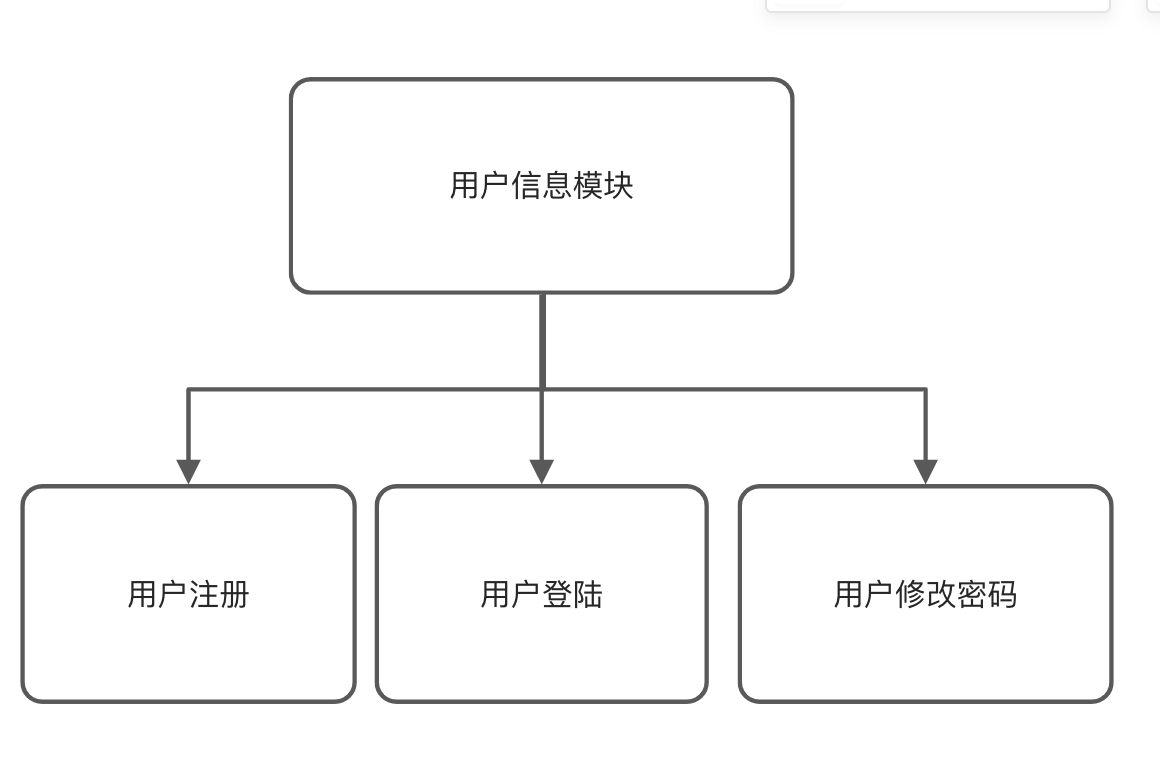
\includegraphics[width=\linewidth,height=9cm]{./assets/user.png}
\subsection{家居管理模块}
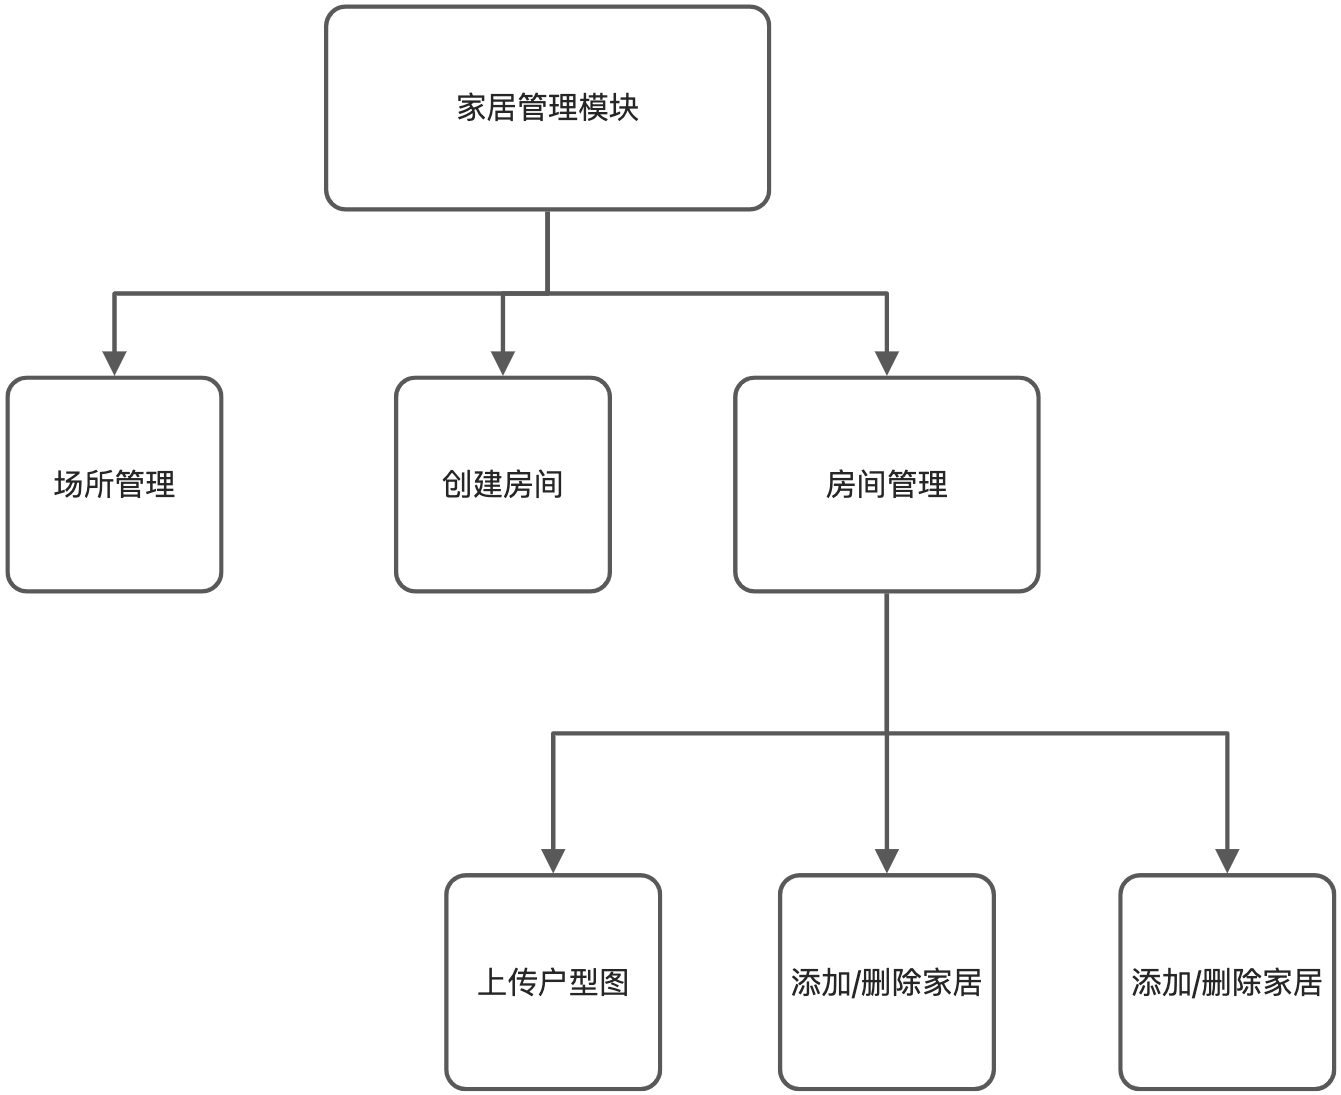
\includegraphics[width=\linewidth,height=10cm]{./assets/jiajuguanli.jpg}
\subsection{客户端项目层次结构}
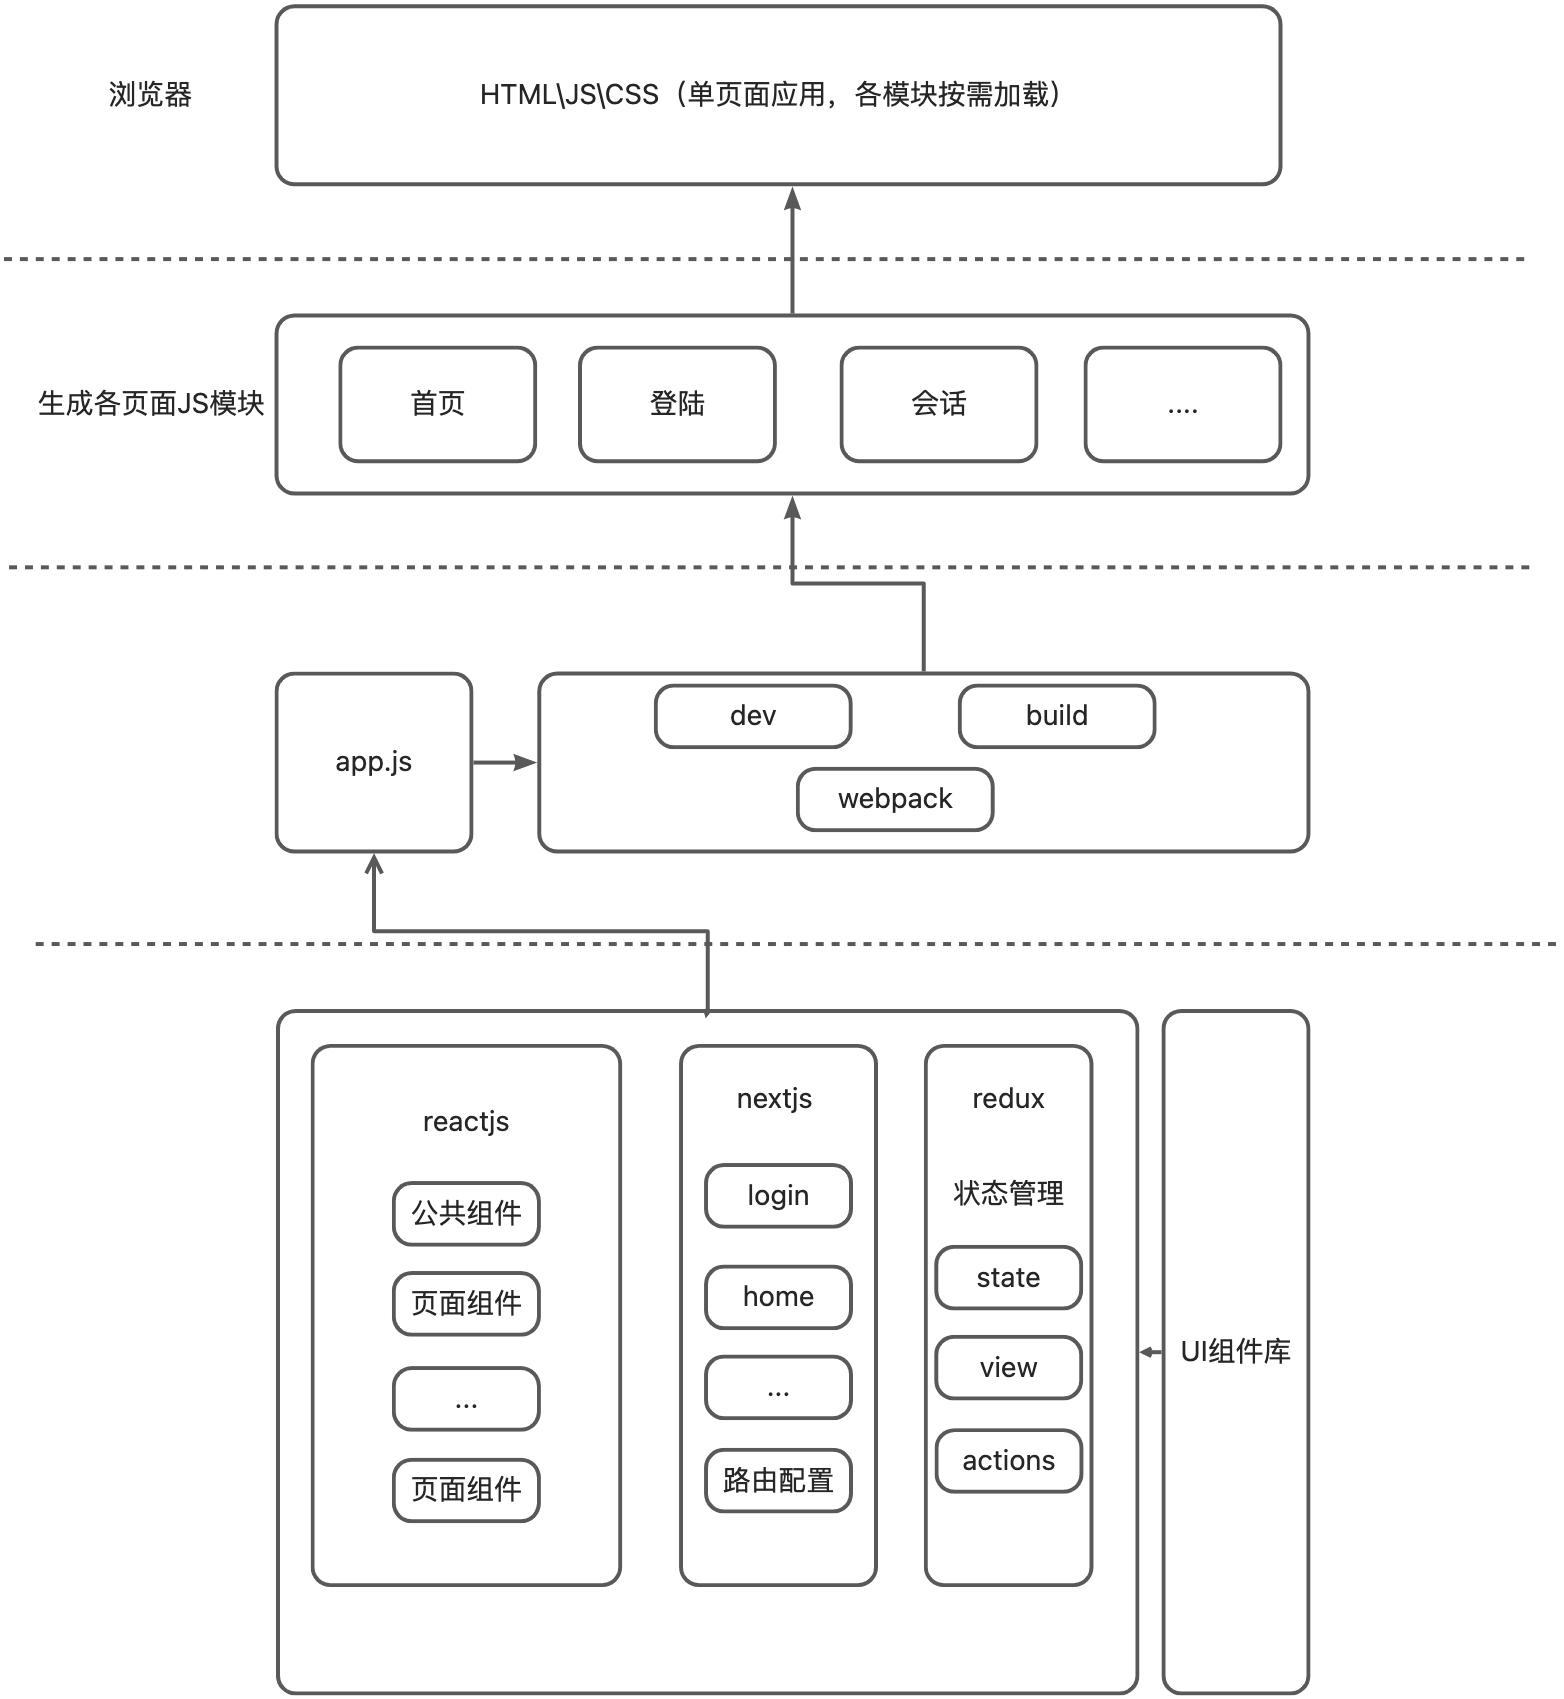
\includegraphics[width=\linewidth]{./assets/client.jpg}
\subsection{服务端项目层次结构}
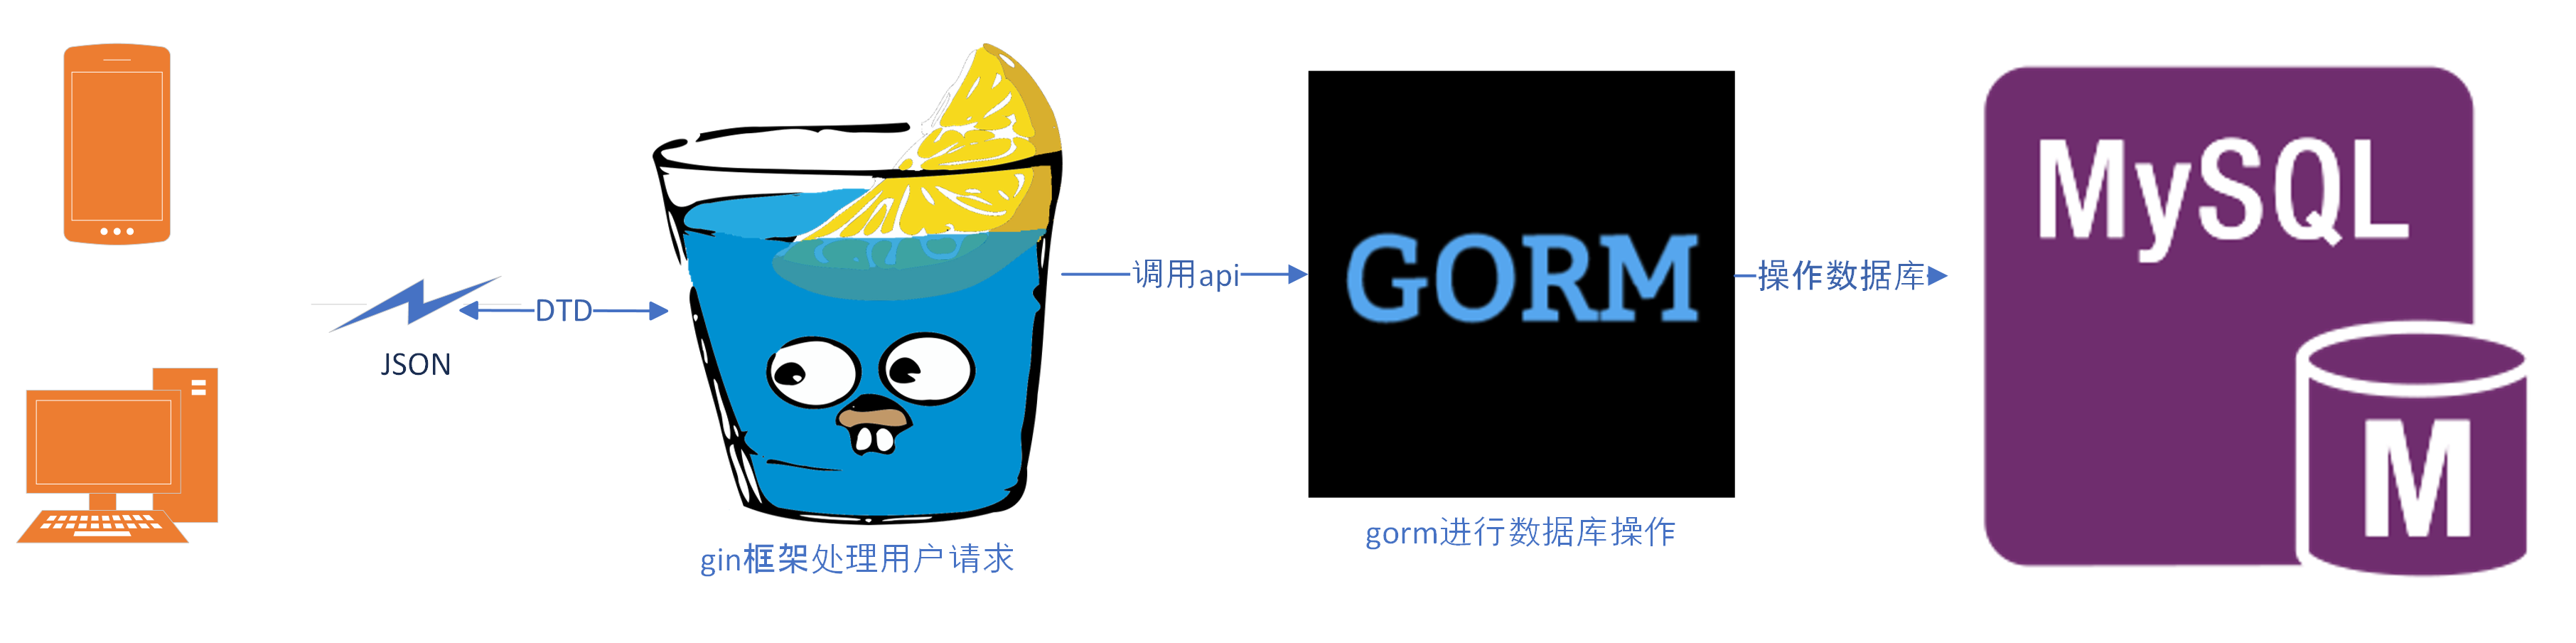
\includegraphics[width=\linewidth]{./assets/server.png}
\section{类图}
\includegraphics*[width=\linewidth]{./assets/devices.png}
\section{数据字典}
\subsection*{users表}
\begin{itemize}
    \item 该表用来存储用户信息
\end{itemize}
\paragraph{}

\end{document}